\chapter{Density Functions}

\section{Multivariate Gaussian}

\begin{equation}
    p(\mathbf{x}) = \frac{1}{\sqrt{(2\pi)^n |\boldsymbol{\Sigma}|}} \exp\left(-\frac{1}{2} (\mathbf{x} - \boldsymbol{\mu})^T \boldsymbol{\Sigma}^{-1} (\mathbf{x} - \boldsymbol{\mu})\right)
    \label{eq:mvn}
\end{equation}

\section{Log Multivariate Gaussian}

\begin{equation}
    \log p(\mathbf{x}) = -\frac{n}{2} \log(2\pi) - \frac{1}{2} \log |\boldsymbol{\Sigma}| - \frac{1}{2} (\mathbf{x} - \boldsymbol{\mu})^T \boldsymbol{\Sigma}^{-1} (\mathbf{x} - \boldsymbol{\mu})
    \label{eq:log_mvn}
\end{equation}


\chapter{Additional Experiment Results}

% \begin{figure}[H]
%     \centering
%     \begin{subfigure}[b]{0.7\textwidth} 
%         \centering
%         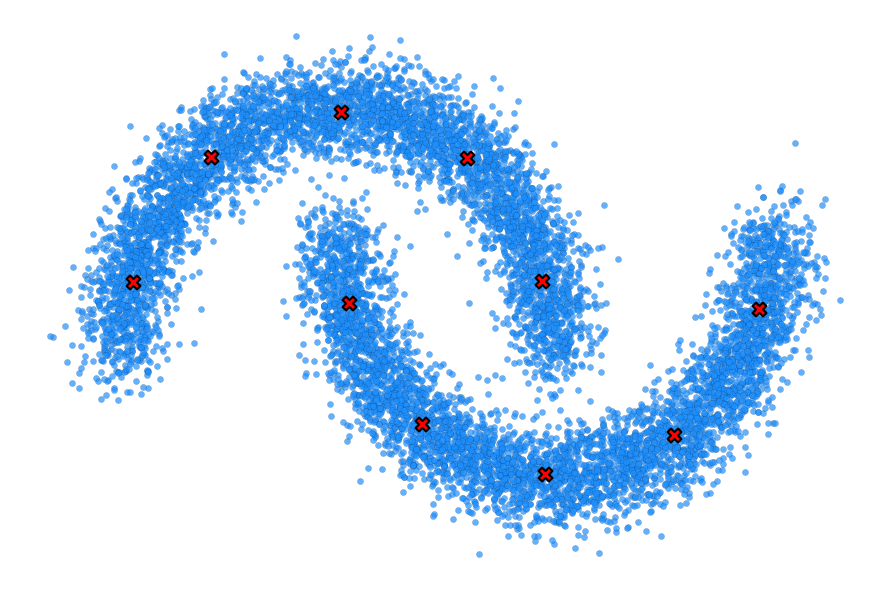
\includegraphics[width=\textwidth]{figures/halfmoons/10_kmeans_data.png}
%         \caption{Initialization}
%     \end{subfigure}
%     \vskip 10pt
%     \begin{subfigure}[b]{0.8\textwidth} 
%         \centering
%         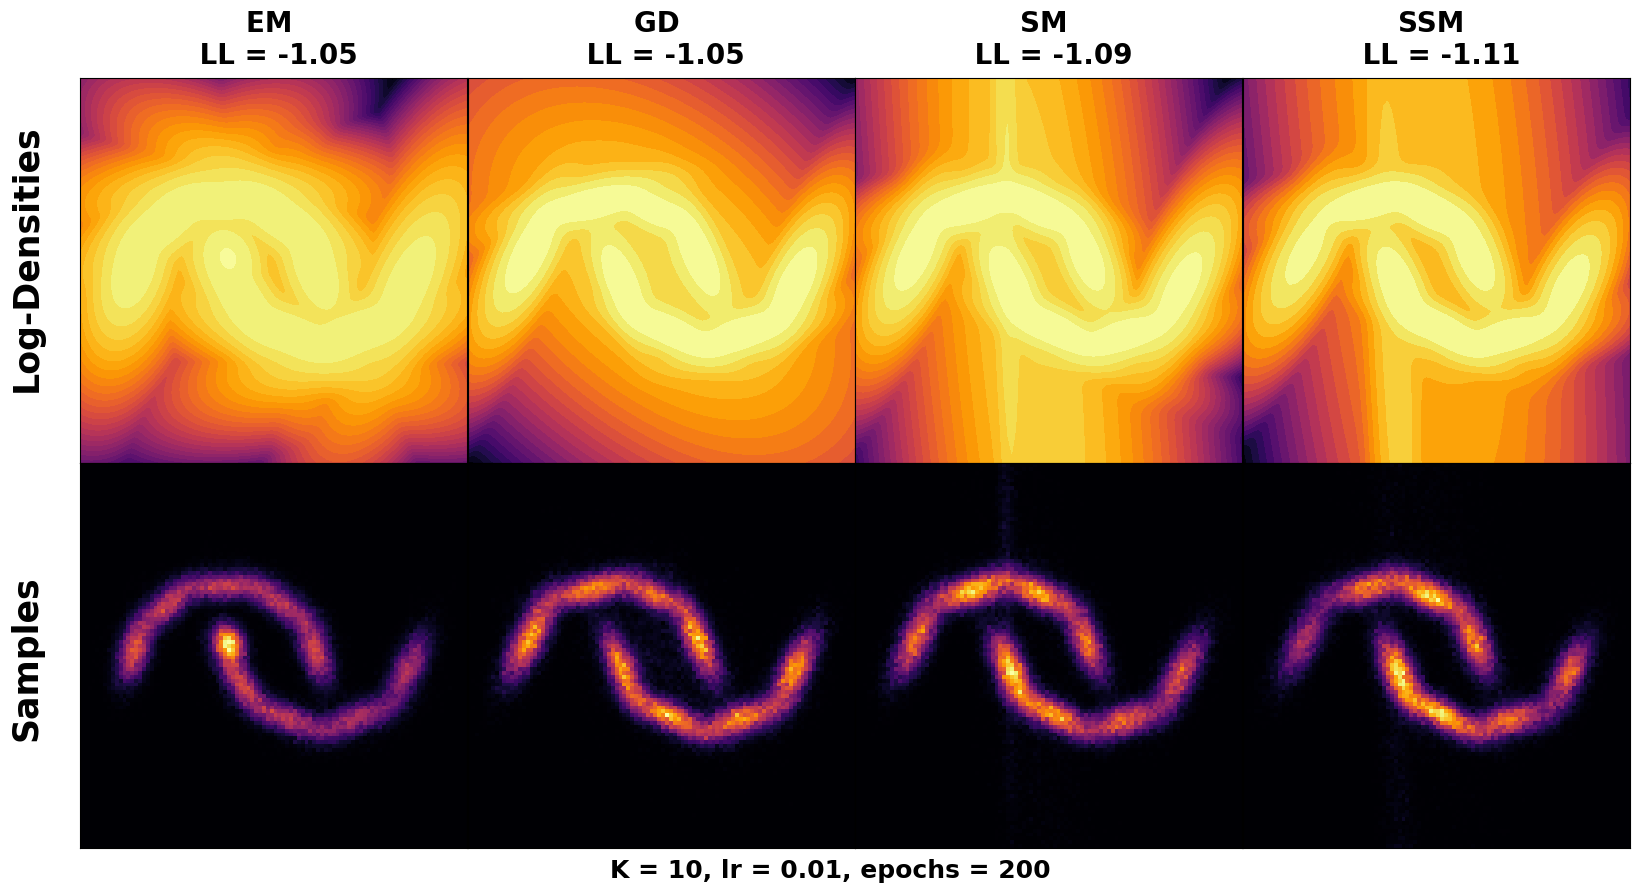
\includegraphics[width=\textwidth]{figures/halfmoons/10_kmeans.png} 
%         \caption{Densities and Samples}
%     \end{subfigure} 
%     \caption{KMeans}
%     \label{fig:kmeans_vs_rand}
% \end{figure}

% \begin{figure}[H]
%     \centering
%     \begin{subfigure}[b]{0.4\textwidth} 
%         \centering
%         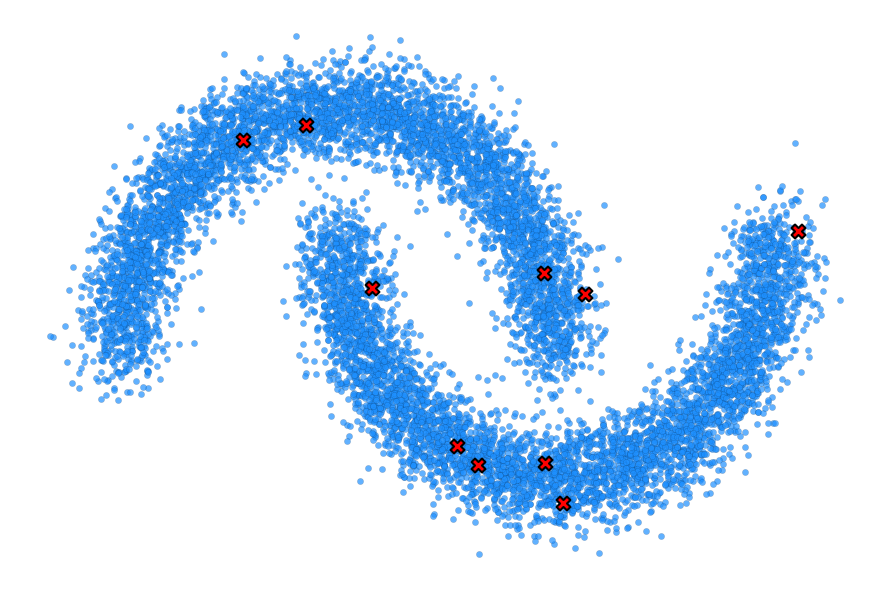
\includegraphics[width=\textwidth]{figures/halfmoons/10_random1_data.png}
%         \caption{Initialization}
%     \end{subfigure}
%     \hfill
%     \begin{subfigure}[b]{0.59\textwidth} 
%         \centering
%         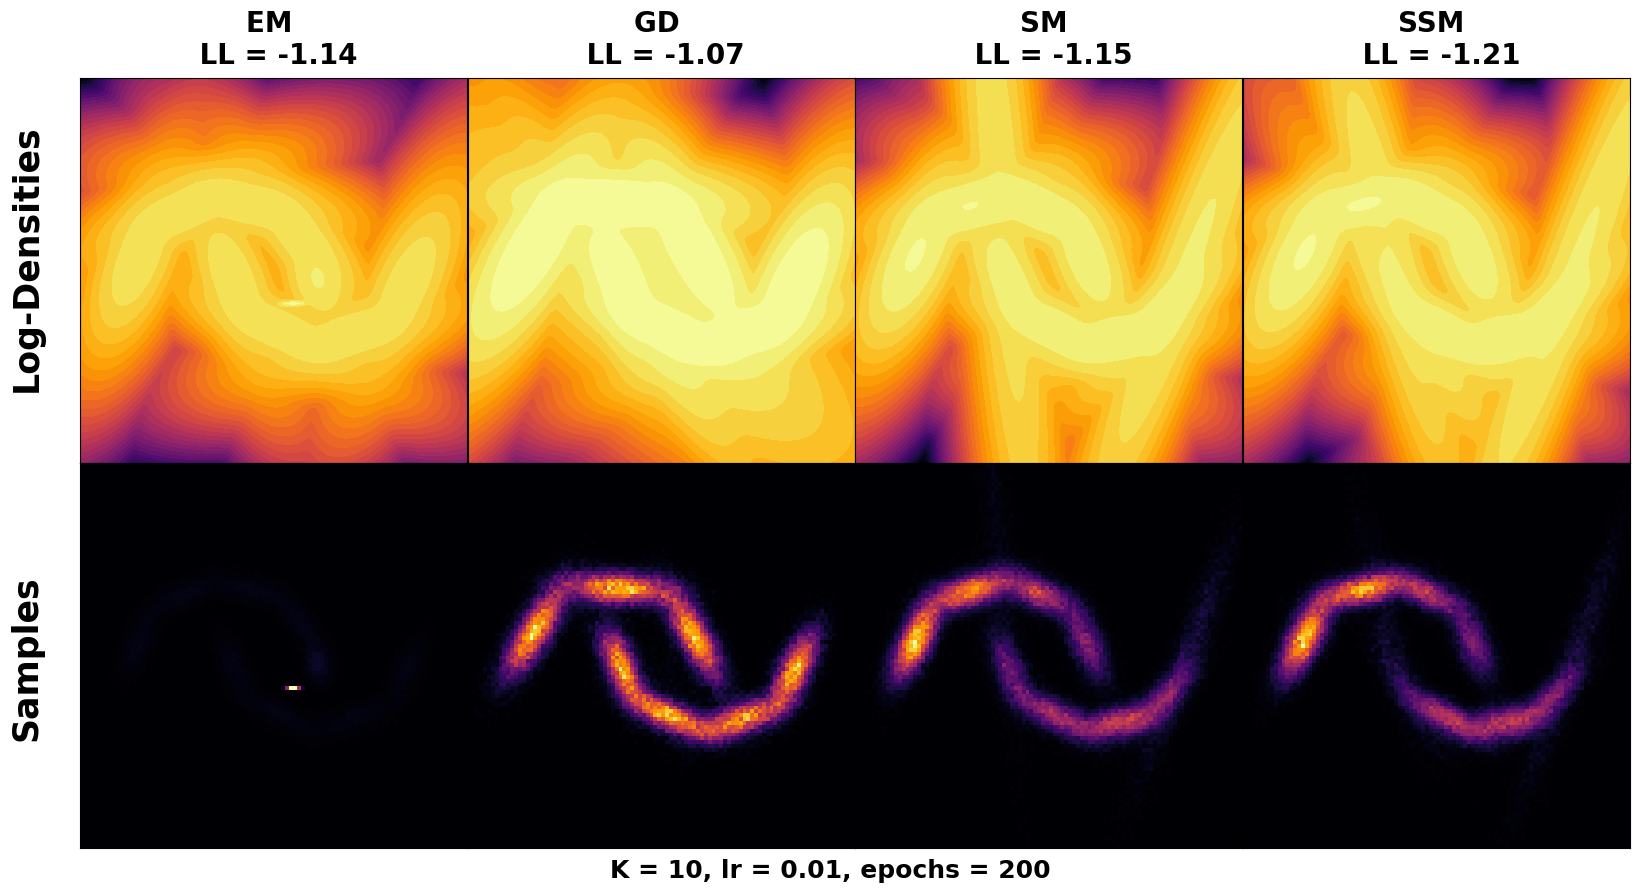
\includegraphics[width=\textwidth]{figures/halfmoons/10_random1.png} 
%         \caption{Densities and Samples}
%     \end{subfigure} 
%     \caption{Random Example 1}
%     \label{fig:kmeans_vs_rand}
% \end{figure}

% \begin{figure}[H]
%     \centering
%     \begin{subfigure}[b]{0.4\textwidth} 
%         \centering
%         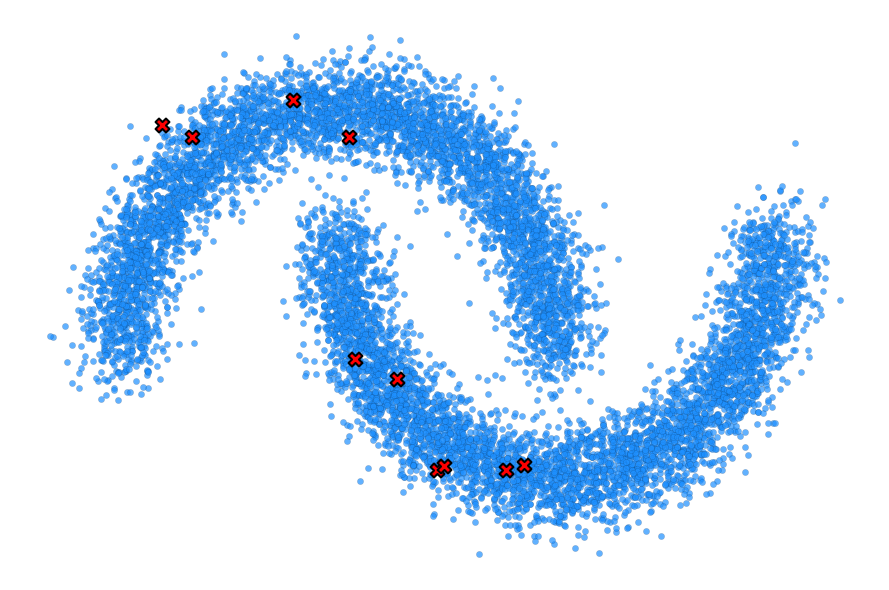
\includegraphics[width=\textwidth]{figures/halfmoons/10_random2_data.png}
%         \caption{Initialization}
%     \end{subfigure}
%     \hfill
%     \begin{subfigure}[b]{0.59\textwidth} 
%         \centering
%         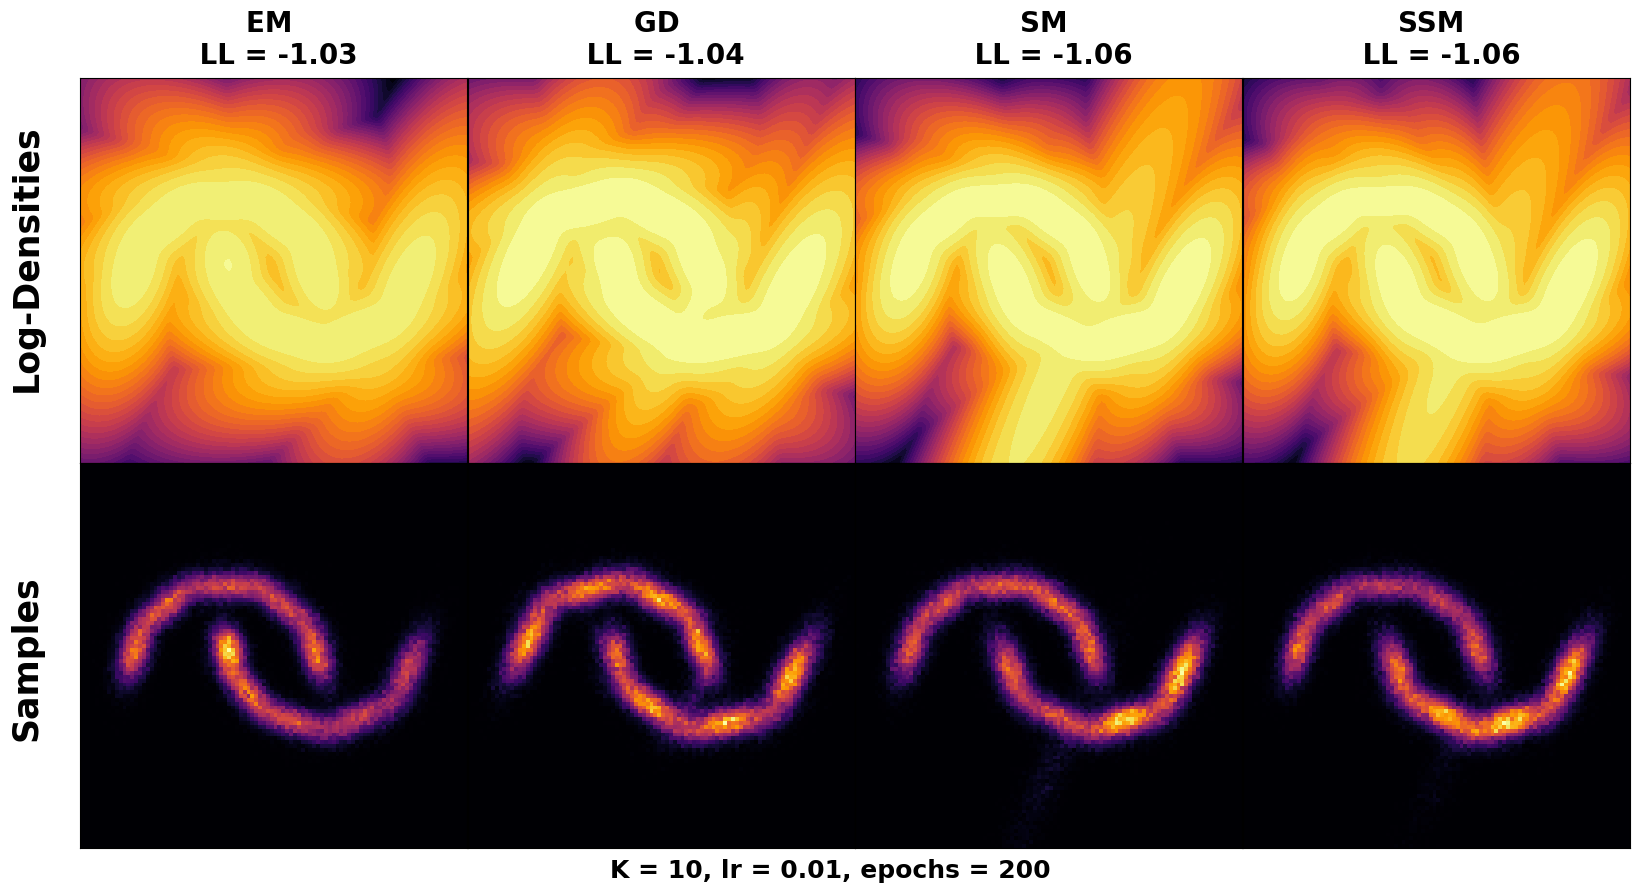
\includegraphics[width=\textwidth]{figures/halfmoons/10_random2.png} 
%         \caption{Densities and Samples}
%     \end{subfigure} 
%     \caption{Random Example 2}
%     \label{fig:kmeans_vs_rand}
% \end{figure}

% \begin{figure}[H]
%     \centering
%     \begin{subfigure}[b]{0.4\textwidth} 
%         \centering
%         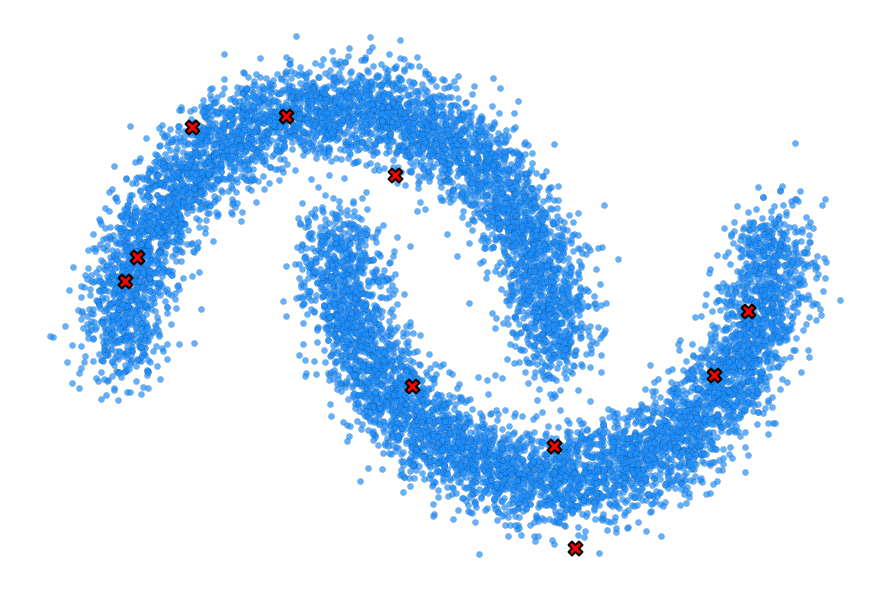
\includegraphics[width=\textwidth]{figures/halfmoons/10_random3_data.png}
%         \caption{Initialization}
%     \end{subfigure}
%     \hfill
%     \begin{subfigure}[b]{0.59\textwidth} 
%         \centering
%         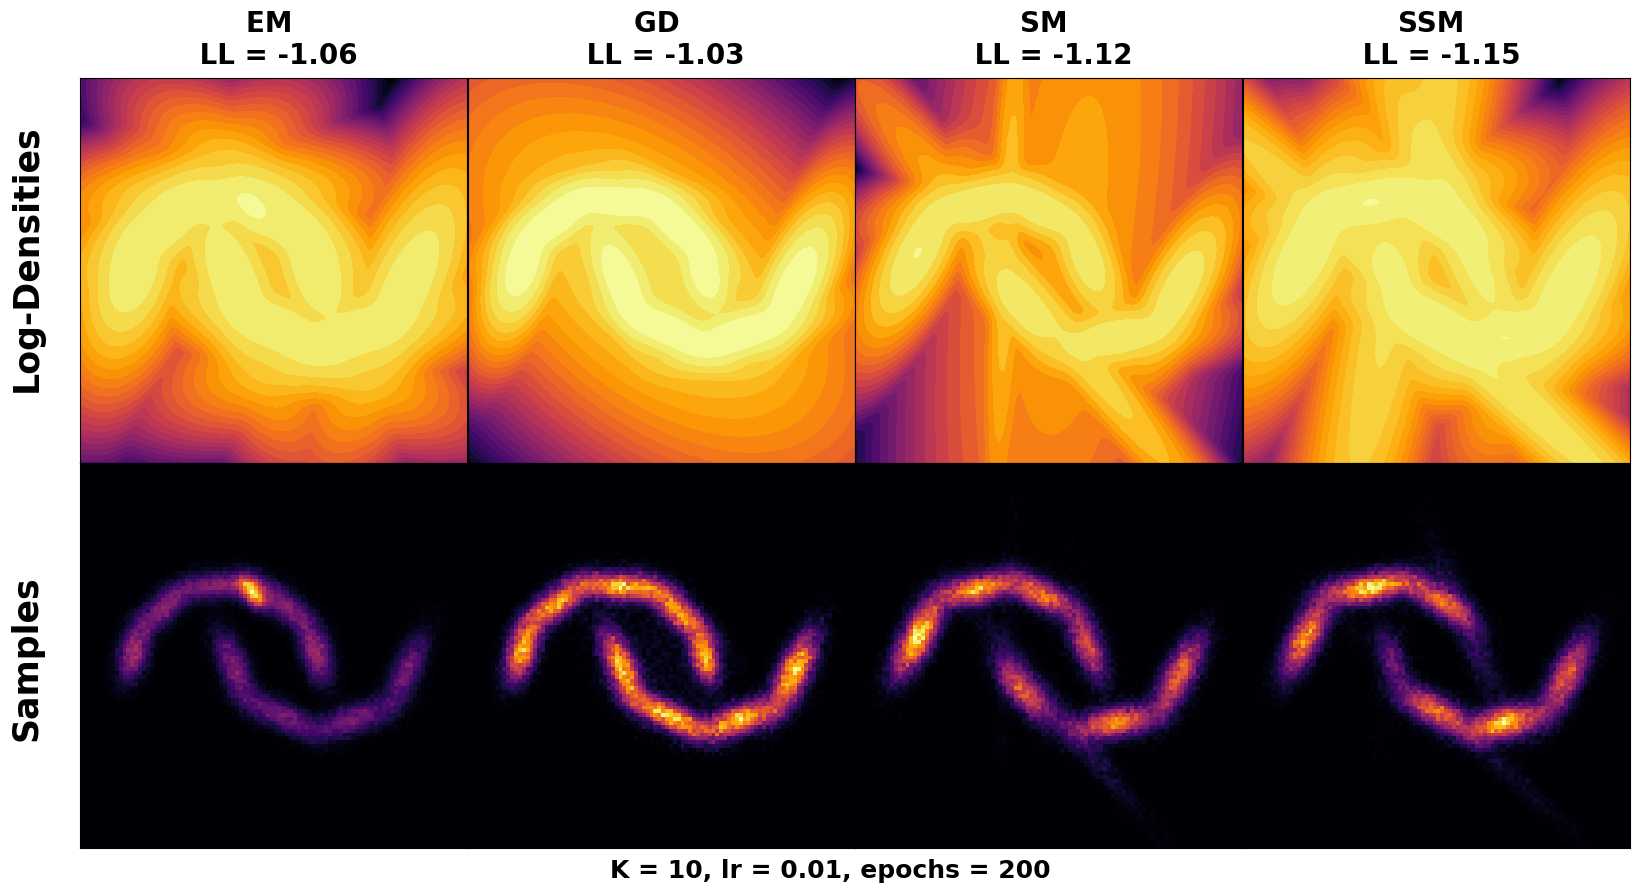
\includegraphics[width=\textwidth]{figures/halfmoons/10_random3.png} 
%         \caption{Densities and Samples}
%     \end{subfigure} 
%     \caption{Random Example 3}
%     \label{fig:kmeans_vs_rand}
% \end{figure}
    
% \begin{figure}[H]
%     \centering
%     \makebox[\textwidth][c]{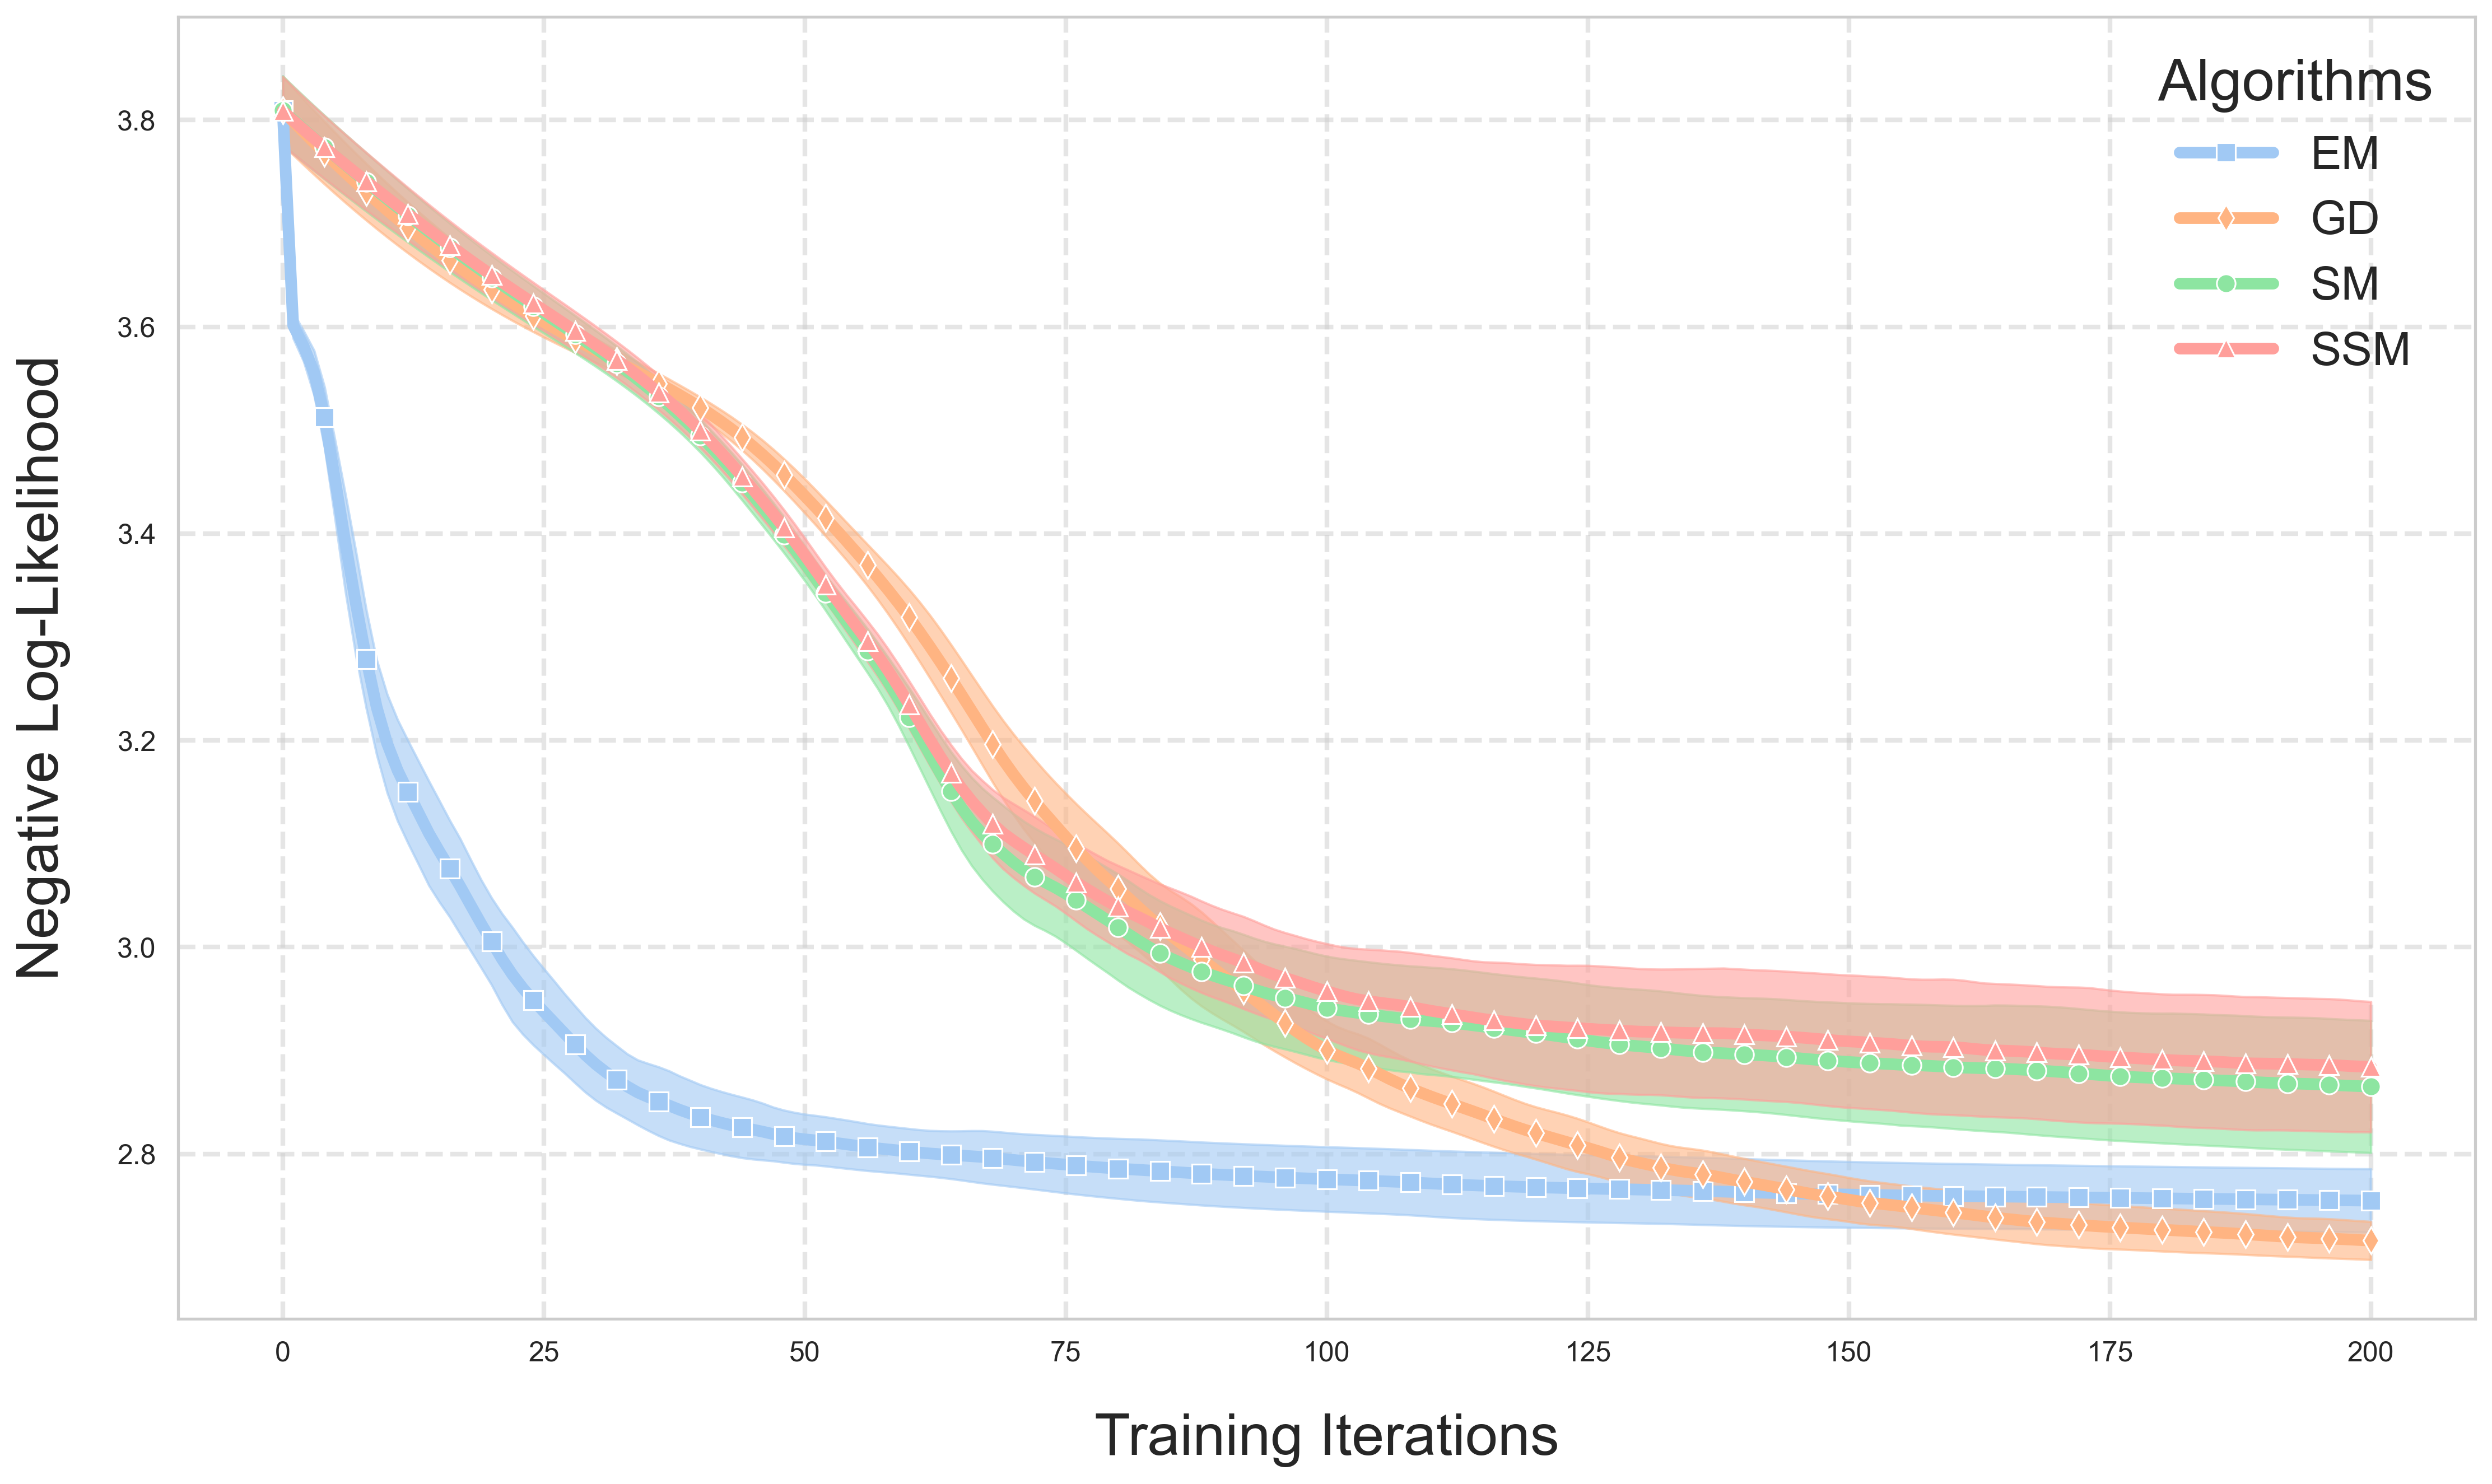
\includegraphics[width=0.9\textwidth]{figures/spirals/30_random_logp.png}}
%     \caption{Negative Log Likelihood over Epochs with random parameter initialization}
%     \label{fig:halfmoons_10_random_logp}
% \end{figure}